% THIS IS SIGPROC-SP.TEX - VERSION 3.1
% WORKS WITH V3.2SP OF ACM_PROC_ARTICLE-SP.CLS
% APRIL 2009
%
% It is an example file showing how to use the 'acm_proc_article-sp.cls' V3.2SP
% LaTeX2e document class file for Conference Proceedings submissions.
% ----------------------------------------------------------------------------------------------------------------
% This .tex file (and associated .cls V3.2SP) *DOES NOT* produce:
%       1) The Permission Statement
%       2) The Conference (location) Info information
%       3) The Copyright Line with ACM data
%       4) Page numbering
% ---------------------------------------------------------------------------------------------------------------
% It is an example which *does* use the .bib file (from which the .bbl file
% is produced).
% REMEMBER HOWEVER: After having produced the .bbl file,
% and prior to final submission,
% you need to 'insert'  your .bbl file into your source .tex file so as to provide
% ONE 'self-contained' source file.
%
% Questions regarding SIGS should be sent to
% Adrienne Griscti ---> griscti@acm.org
%
% Questions/suggestions regarding the guidelines, .tex and .cls files, etc. to
% Gerald Murray ---> murray@hq.acm.org
%
% For tracking purposes - this is V3.1SP - APRIL 2009

\documentclass{acm_proc_article-sp}

\begin{document}

\title{Efficient Data-Intensive Computing\titlenote{(Does NOT produce the permission block, copyright information nor page numbering). For use with ACM\_PROC\_ARTICLE-SP.CLS. Supported by ACM.}}
\subtitle{Do we want a subtitle?
\titlenote{A full version of this paper is available as
\textit{Author's Guide to Preparing ACM SIG Proceedings Using
\LaTeX$2_\epsilon$\ and BibTeX} at
\texttt{www.acm.org/eaddress.htm}}}
%
% You need the command \numberofauthors to handle the 'placement
% and alignment' of the authors beneath the title.
%
% For aesthetic reasons, we recommend 'three authors at a time'
% i.e. three 'name/affiliation blocks' be placed beneath the title.
%
% NOTE: You are NOT restricted in how many 'rows' of
% "name/affiliations" may appear. We just ask that you restrict
% the number of 'columns' to three.
%
% Because of the available 'opening page real-estate'
% we ask you to refrain from putting more than six authors
% (two rows with three columns) beneath the article title.
% More than six makes the first-page appear very cluttered indeed.
%
% Use the \alignauthor commands to handle the names
% and affiliations for an 'aesthetic maximum' of six authors.
% Add names, affiliations, addresses for
% the seventh etc. author(s) as the argument for the
% \additionalauthors command.
% These 'additional authors' will be output/set for you
% without further effort on your part as the last section in
% the body of your article BEFORE References or any Appendices.

\numberofauthors{8} %  in this sample file, there are a *total*
% of EIGHT authors. SIX appear on the 'first-page' (for formatting
% reasons) and the remaining two appear in the \additionalauthors section.
%
\author{
% You can go ahead and credit any number of authors here,
% e.g. one 'row of three' or two rows (consisting of one row of three
% and a second row of one, two or three).
%
% The command \alignauthor (no curly braces needed) should
% precede each author name, affiliation/snail-mail address and
% e-mail address. Additionally, tag each line of
% affiliation/address with \affaddr, and tag the
% e-mail address with \email.
%
% 1st. author
\alignauthor
Ben Trovato\titlenote{Dr.~Trovato insisted his name be first.}\\
       \affaddr{Institute for Clarity in Documentation}\\
       \affaddr{1932 Wallamaloo Lane}\\
       \affaddr{Wallamaloo, New Zealand}\\
       \email{trovato@corporation.com}
% 2nd. author
\alignauthor
G.K.M. Tobin\titlenote{The secretary disavows
any knowledge of this author's actions.}\\
       \affaddr{Institute for Clarity in Documentation}\\
       \affaddr{P.O. Box 1212}\\
       \affaddr{Dublin, Ohio 43017-6221}\\
       \email{webmaster@marysville-ohio.com}
% 3rd. author
\alignauthor Lars Th{\o}rv{\"a}ld\titlenote{This author is the
one who did all the really hard work.}\\
       \affaddr{The Th{\o}rv{\"a}ld Group}\\
       \affaddr{1 Th{\o}rv{\"a}ld Circle}\\
       \affaddr{Hekla, Iceland}\\
       \email{larst@affiliation.org}
\and  % use '\and' if you need 'another row' of author names
% 4th. author
\alignauthor Lawrence P. Leipuner\\
       \affaddr{Brookhaven Laboratories}\\
       \affaddr{Brookhaven National Lab}\\
       \affaddr{P.O. Box 5000}\\
       \email{lleipuner@researchlabs.org}
% 5th. author
\alignauthor Sean Fogarty\\
       \affaddr{NASA Ames Research Center}\\
       \affaddr{Moffett Field}\\
       \affaddr{California 94035}\\
       \email{fogartys@amesres.org}
% 6th. author
\alignauthor Charles Palmer\\
       \affaddr{Palmer Research Laboratories}\\
       \affaddr{8600 Datapoint Drive}\\
       \affaddr{San Antonio, Texas 78229}\\
       \email{cpalmer@prl.com}
}
% There's nothing stopping you putting the seventh, eighth, etc.
% author on the opening page (as the 'third row') but we ask,
% for aesthetic reasons that you place these 'additional authors'
% in the \additional authors block, viz.
\additionalauthors{Additional authors: John Smith (The Th{\o}rv{\"a}ld Group,
email: {\texttt{jsmith@affiliation.org}}) and Julius P.~Kumquat
(The Kumquat Consortium, email: {\texttt{jpkumquat@consortium.net}}).}
\date{30 July 1999}
% Just remember to make sure that the TOTAL number of authors
% is the number that will appear on the first page PLUS the
% number that will appear in the \additionalauthors section.

\maketitle
\begin{abstract}
We propose a model for predicting the optimal performance of large-scale parallel dataflow systems based on various hardware and workload parameters. Using this model, we show that existing systems, such as Google's MapReduce \cite{mapreduce}, Hadoop \cite{hadoop} and Dryad \cite{dryad}, are highly inefficient, often exhibiting throughput that is more than ten times less than the predicted optimal throughput for the same hardware and workload. By implementing Parallel DataSeries, an efficient open-source parallel dataflow system, we show that with careful engineering it is possible to achieve near-optimal performance.

We also discuss the \emph{data exchange wall}, a phenomenon in which the overall throughput drops when a data-parallel program is executed on a parallel dataflow system spanning multiple nodes (ie, machines). As a result of current industry trends towards higher intra-node parallelism (via multiple CPU cores and GPGPUs \cite{cuda, stream, opencl}), the data exchange wall will need to be strongly considered in any data-intensive computing work.
\end{abstract}

% A category with the (minimum) three required fields
\category{H.4}{Information Systems Applications}{Miscellaneous}
%A category including the fourth, optional field follows...
\category{D.2.8}{Software Engineering}{Metrics}[complexity measures, performance measures]

\terms{Delphi theory}

\keywords{ACM proceedings, \LaTeX, text tagging} % NOT required for Proceedings

\section{Introduction}
Large-scale parallel dataflow systems, such as MapReduce \cite{mapreduce} and Dryad \cite{dryad}, have attracted significant attention recently. They provide abstractions for specifying data-parallel computations, and they also provide environments for automating the execution of data-parallel programs on large clusters of commodity machines. MapReduce, in particular, has received a great deal of attention, and several implementations \cite{hadoop, phoenix} are publicly available. These programming models and systems offer an alternative to parallel databases \cite{paralleldatabases} for processing large data sets.

Although existing systems can scale to hundreds and thousands of machines, they do not fully utilize the hardware resources on which they execute. Google's MapReduce implementation reached a peak input data transfer rate of only 30 GB/s while running a distributed grep on a cluster of 1800 two-disk nodes. That rate is equivalent to only 8.33 MB/s per disk at the peak, which is only reached 60 seconds into the computation. As another example, Hadoop completed \cite{hadoop2009} the TeraByte Sort benchmark \cite{sortbenchmark} in 62 seconds on a cluster of 1406 four-disk nodes, obtaining an average throughput of only 11.47 MB/s per node, or 2.87 MB/s per disk. These observations indicate that many organizations and individuals are spending excessive resources to run their data-parallel programs (purchasing or renting unnecessary hardware, maintaining the system, etc.).

Existing parallel dataflow systems have achieved scalability while exhibiting poor efficiency and underutilization of hardware resources. Although scalability is critical because it enables users to tackle large problems in ``reasonable'' time, users of such systems would benefit from higher efficiency. Unfortunately, there are no publicly available models that help users understand the bottlenecks of their parallel dataflow systems and data-parallel programs. The lack of such models affects different users in different ways. For example:
\begin{itemize}
  \item Developers of parallel dataflow systems do not know where to focus their development efforts. Should they invest in optimizing the local (ie, per-node) performance of their systems (eg, the throughput of the sorting phase in a map-reduce system, such as Hadoop) or, instead, focus on reducing the typical amount of inter-rack data exchange?
  \item Developers of programs that run on parallel dataflow systems do not know whether they should spend time optimizing the local (ie, per-node) performance of their programs (eg, the map function in a map-reduce computation) or, instead, focus on reducing the amount of data exchange (ie, network traffic).
  \item Administrators do not know what hardware configuration would provide the best performance for their organizations' workloads. Would it be beneficial to increase the number of CPUs or the number of disks per node, or perhaps purchase a single, powerful node instead of a cluster of inexpensive nodes? Would it be beneficial to use Infiniband rather than Gigabit Ethernet? What is the impact of running on Amazon EC2 \cite{amazonec2} platform, where the network is generally slower?
\end{itemize}

This paper makes several contributions. First, we provide a simple model for predicting the optimal performance of a parallel dataflow system based on various hardware and workload parameters. This model will help developers and administrators answer the preceding questions. Second, we analyze the conditions under which the network limits the effective ``throughput per node'' (we call this condition the \emph{data exchange wall}). Third, we show that existing parallel dataflow systems are highly inefficient. Finally, we present Parallel DataSeries, an efficient open-source parallel dataflow system that is far more efficient than existing systems.

\section{Efficiency Model}

In this section we analyze the dataflow of a parallel dataflow system, focusing on map-reduce systems. First, we provide a high-level overview of the dataflow. Then, we provide a more detailed analysis of the parallelism in the map-reduce dataflow, including both partitioned parallelism and pipelined parallelism. We also argue that processing (ie, CPU) time can be ignored due to pipelined parallelism. Finally, we provide a set of simple mathematical formulas for calculating the optimal execution time of a data-parallel program on a parallel dataflow system. Although these formulas are specific to systems/programs with two phases, such as map-reduce, they can be easily extended to support an arbitrary number of phases.

\subsection{Map-Reduce Dataflow}

In parallel dataflow systems, data is read from input files, then processed and finally stored in output files. The system is organized as a pipeline, in which the output of one operator is the input of the following step.

\begin{figure*}
\begin{center}
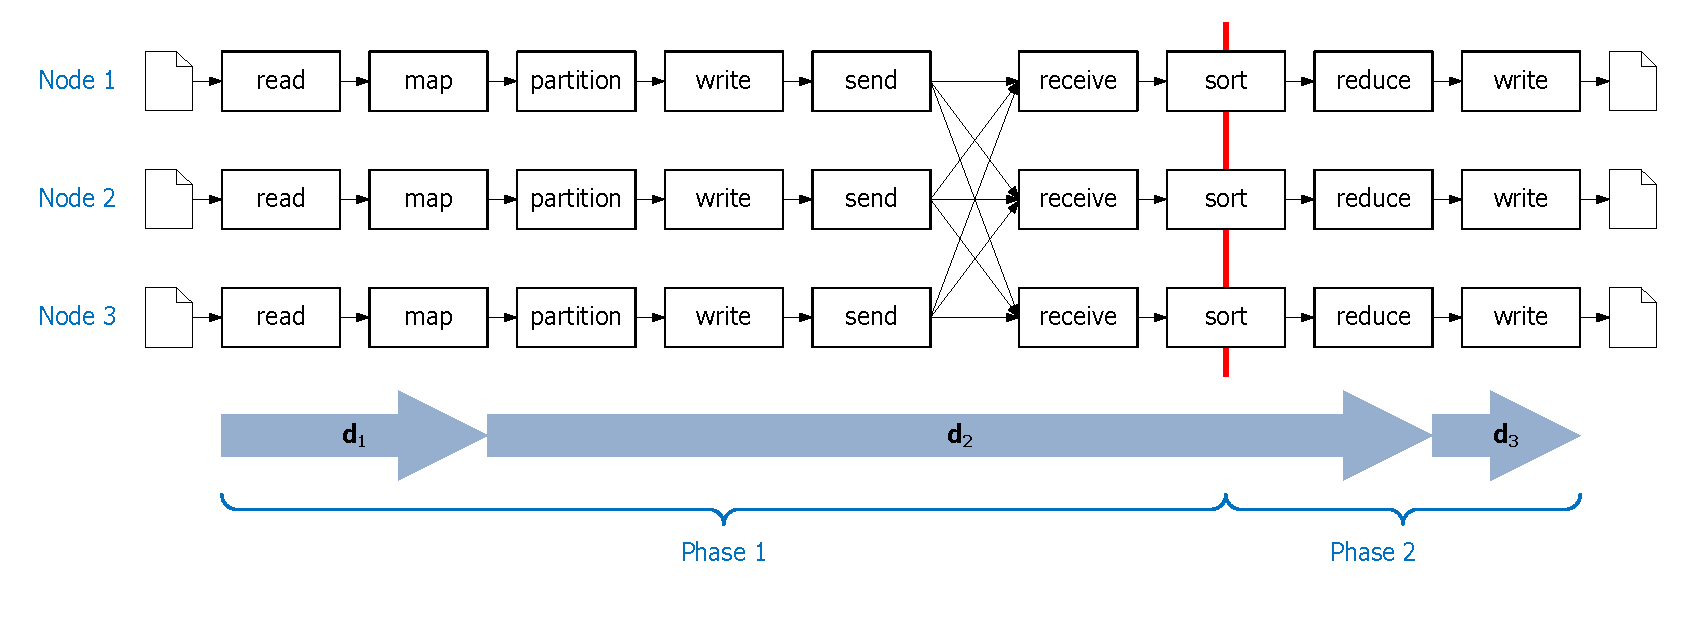
\epsfig{width=7in, angle=0, file=fig/mapreduce.ps}
\caption{A map-reduce dataflow.}
\label{fig:mapreduce}
\end{center}
\end{figure*}

Figure \ref{fig:mapreduce} illustrates the pipeline of a typical map-reduce computation involving three nodes. The computation is divided into two phases, labeled Phase 1 and Phase 2, where each phase consists of steps that can execute in parallel, as explained in the following section.

The first write step in Figure \ref{fig:mapreduce} is responsible for writing the output of the map step to persistent storage. Although this step is not required in order to perform a map-reduce computation, it increases the system's ability to cope with failures. Without this mechanism, if a single reduce task crashes, all of the map tasks must be re-executed. When running a long computation on a large cluster, where it is likely that one of the nodes will fail during the computation, it is a good idea to include this step. However, if the total number of ``machine hours'' required for a computation is small, the performance benefit from omitting this step probably outweighs the cost of having to re-run the computation if one of the nodes fails during the original computation.

In some map-reduce implementations, such as Google's MapReduce and Hadoop, the output of the map step is written to disk and then read back from disk before sending the data over the network. This approach is inefficient because it involves the unnecessary step of reading the entire data from disk.

It is also worth noting that parallel dataflow systems often utilize underlying distributed file systems, such as GFS \cite{gfs}, in which a node's input data may reside on a different node, but in most cases such systems are able to schedule the map tasks so that input data is read from the local disks \cite{mapreduce}.

Figure \ref{fig:mapreduce} also illustrates how the amount of data ``flowing'' through the system changes throughout the computation. The amount of input data per node is $d_1$, and the amount of output data per node is $d_3$. The amount of data per node produced by the map step and consumed by the reduce step is $d_2$. In most applications, the amount data flowing through the system either remains the same or decreases (ie, $d_1 \ge d_2 \ge d_3$). For example, in a distributed ``grep'' computation, $d_1 > d_2$ and $d_2 = d_3$. In a distributed sort computation there is no data reduction, so $d_1 = d_2 = d_3$.

\subsection{Dataflow Parallelism}

In this section we discuss the two forms of parallelism that occur in a parallel-dataflow system: partitioned parallelism and pipelined parallelism. We then explain why processing time (aka CPU time) can be ignored in the context of typical data-parallel programs running on an efficient parallel dataflow system.

DeWitt and Gray \cite{paralleldatabases} divide the potential parallelism in a database system into partitioned parallism and pipelined parallelism. A data-parallel program running on a parallel dataflow system is similar to a relational query in a database in that it consists of operators applied to streams of data. Partitioned parallelism is achieved by partitioning the data and splitting an operator into multiple operators running on different ``processors.'' Pipelined parallelism, on the other hand, is achieved by streaming the output of one operator into the input of another operator so that the two operators can work in series.

Figure \ref{fig:mapreduce} outlines partitioned parallelism and pipelined parallelism in a map-reduce computation. Partitioned parallelism takes place on the vertical axis. The input data is split between three nodes, and each operator (eg, read, map) is, in fact, split into three sub-operators. Each of the three sub-operators runs on a different node, thereby providing partitioned parallelism. The primary focus of previous work on parallel dataflow systems has been on providing large-scale partitioned parallelism.

Pipelined parallelism takes place on the horizontal axis of Figure \ref{fig:mapreduce}. Specifically, the operators in each phase take advantage of pipelined parallelism, whereas pipelined parallelism cannot occur between operators in different phases.

As an example, the read operator is responsible for reading input data from disk. The data is read from disk as a stream, so each record that is read from disk can be immediately passed to the map operator, which can convert (ie, ``map'') that record into zero or more records, which are then passwed to the partition operator, and so forth. In other words, the map operator does not need to wait for all of the input to be read from disk, and the partition operator does not need to wait for the map operator to finish operating on all of the records. The only operator in Figure \ref{fig:mapreduce} that does not support pipelined parallelism is the sort operator. The sort operator can only produce its first output record after it has received all of its input records. (The last input record might be the first in sorted order.)

The sort operator itself is actually a series of soperators, so it is helpful to zoom into the details. There are two variants of the sort operator. One performs in-memory sorting, and is used if the data to be sorted fits in memory. The other performs an external (aka two-pass) sort, and is used if the data to be sorted does not fit in memory.

\begin{figure}
\epsfig{width=3.2in, angle=0, file=fig/sort.ps}
\caption{The sub-operators of the sort step. Left: Our in-memory sort first arranges the records in buckets, then sorts the buckets individually and finally copies (ie, gathers) the records into contiguous blocks of memory. Right: An external sort involves sorting batches of records, writing each batch to disk, and finally merging the files to produce a sorted stream of records.}
\label{fig:sort}
\end{figure}

Our implementation of in-memory sorting in Parallel DataSeries included three operators, as shown on the left side of \ref{fig:sort}:
\begin{itemize}
  \item Bucket: For each input record, place a pointer to the record in a bucket based on the first few bytes of the key field.
  \item Sort buckets: Sort each bucket using a standard quicksort algoritm.
  \item Gather: Iterate through all of the buckets and pointers in sorted order, and copy the actual records into contiguous memory.
\end{itemize}

Our in-memory sorting strategy, which consists of three operators, allows us to pipeline most of the work with other operators in the overall map-reduce computation. The bucket operator can be pipelined with Phase 1, whereas the gather operator can be pipelined with Phase 2. The only actual operator that cannot be pipelined with other operators is the sort buckets operator. However, this operator offers the opportunity for partitioned parallelism within the node by dividing the buckets among the CPU cores on the node. With four cores, we were able to sort 10 million 100-byte records, divided into $2^{16}$ buckets, in 0.3 seconds. That is, the sort buckets operator achieved a throughput of 33.33 million records per second, or 3.3 GB/s.

Our implementation of external sorting in Parallel DataSeries included four operators, as shown on the right side of Figure \ref{fig:sort}:
\begin{itemize}
  \item In-memory sort: This operator consumes as much data as it can fit into memory, and then sorts it using the three operators of the in-memory sorting described earlier.
  \item Write: Each memory-size batch of data is written to a file on disk
  \item Read: The sorted files are read from disk. The merge operator decides which file to read next, and how many records to read from it.
  \item Merge: The records from the files are merged into one long sorted stream.
\end{itemize}

One interesting aspect of the external sort is that it includes an operator (in-memory sort) that is quite different from the typical streaming operator. The in-memory sort, as described earlier, actually consists of three operators and cannot offer pipelined parallelism. However, in the context of an external sort, in which the amount of data per node after the map operation is significantly greater than the amount of memory available on a node, we can actually achieve pipelined parallelism in the in-memory sort operator (but at a courser granularity). For instance, if we consider the stream of records flowing into the sort operator in Figure \ref{fig:mapreduce}, and we divide it into batches where the size of each batch is slightly less than 50\% of the node's available memory, then the bucket operator can operate on one batch while the gather operator is opereating on the previous batch. There is some loss of pipelined parallelism in the first and last batches, but if there is a sufficient amount of data to sort, then this loss can be ignored. 

Our efficiency model is designed to provide a tight lower bound on the execution time of a data-parallel program. From the beginning, it was clear to us that it would be difficult to account for computation in our model. Unlike hard disks and network interfaces, for example, where one can easily determine the sustained throughput (in MB/s), it is much harder to reason about the ``throughput'' of a CPU due to the plethora of architectures, the interaction with other components of the system (eg, caches, memory) and the dependency on the program itself (eg, branches, memory access locality).

Fortunately, all of the CPU-intensive operators -- map, partition, bucket, sort buckets, gather, reduce -- with the exception of sort buckets, take place in pipelined parallelism with operators that read/write from/to disk and send/receive to/from the network. In the vast majority of data-parallel programs and parallel dataflow systems, all of the CPU-intensive operators operate at throughputs that are far greater than that of the I/O intensive operators, so they do not affect the throughput of the computation whatsoever. From our experience, the sort buckets operator, which cannot be pipeline parallelized with other steps, is so fast that it too can be ignore. Furthermore, the sort buckets can be partition parallelized by utilizing multiple cores, and with the growing number of cores per node, this operator will become even more negligible in the future. 

\subsection{Optimal Execution Time}

Referring to Figure \ref{fig:mapreduce}, we can isolate all of the I/O activities that must occur in each of the phases (depending on whether or not an external sort is needed, of course). Table \ref{table:operations1} lists the actual I/O-related operations that take place.

\begin{table}
\centering
\begin{minipage}{0.5\textwidth}
\centering
\renewcommand{\arraystretch}{1.2}
\begin{tabular}{|l|l|l|}
\hline
        & $d_2 < \text{memory}$          & $d_2 \gg \text{memory}$ \\ \hline
Phase 1 & $1 \times$ disk read:  $d_1$   & $1 \times$ disk read:  $d_1$ \\ 
        & $1 \times$ disk write\footnote{This ``backup write'' is optional.}: $d_2$ & $1 \times$ disk write: $d_2$ \\
        & $1 \times$ network: $d_2$      & $1 \times$ network:    $d_2$ \\
        &                                & $1 \times$ disk write: $d_2$ \\ \hline
Phase 2 & $1 \times$ disk write: $d_3$   & $1 \times$ disk read:  $d_2$ \\
        &                                & $1 \times$ disk write: $d_3$ \\ \hline
\end{tabular}
\caption{The I/O-operations in a map-reduce parallel dataflow system.}
\end{minipage}
\label{table:operations1}
\end{table}

Many parallel dataflow systems utilize distributed file systems, such as GFS \cite{gfs} and HDFS \cite{hdfs}. Such file systems typically use replication and store multiple copies of each block of data. In most cases, the tasks of a data-parallel program can be scheduled so that the input data is read locally and does not need to be sent over the network. However, at the end of the last phase, each node must send its output data to $r - 1$ other nodes, where $r$ is the file system's replication factor. The sending node, along with the $r - 1$ receiving nodes, write the data to their their local disks, thereby ensuring that $r$ copies of the data are stored. Obviously, all of these operations occur in parallel (ie, piplelined parallelism) to the other operations of the last phase of the computation. Table \ref{table:operations2} lists the I/O-related operations that take place in a parallel dataflow system that utilizes a distributed file system with $r$-way replication.

\begin{table}
\centering
\begin{minipage}{0.5\textwidth}
\centering
\renewcommand{\arraystretch}{1.2}
\begin{tabular}{|l|l|l|}
\hline
        & $d_2 < \text{memory}$          & $d_2 \gg \text{memory}$ \\ \hline
Phase 1 & $1 \times$ disk read:  $d_1$   & $1 \times$ disk read:  $d_1$ \\ 
        & $1 \times$ disk write\footnote{This ``backup write'' is optional.}: $d_2$ & $1 \times$ disk write: $d_2$ \\
        & $1 \times$ network: $d_2$      & $1 \times$ network:    $d_2$ \\
        &                                & $1 \times$ disk write: $d_2$ \\ \hline
Phase 2 & $\left(r - 1\right) \times$ network: $d_3$ & $1 \times$ disk read:  $d_2$ \\
        & $r \times$ disk write: $d_3$   & $\left(r - 1\right) \times$ network: $d_3$ \\
        &                                & $r \times$ disk write: $d_3$ \\ \hline
\end{tabular}
\caption{The I/O-operations in a map-reduce parallel dataflow system that utilizes a distributed file system with $r$-way replication.}
\end{minipage}
\label{table:operations2}
\end{table}

Following our conclusion that only I/O-intensive operators have a real impact on the execution time of a data-parallel program, we can easily determine the execution time based on Table \ref{table:operations1} and Table \ref{table:operations2}. We use the following symbols:

\begin{table}
\centering
\begin{minipage}{0.5\textwidth}
\centering
\renewcommand{\arraystretch}{1.2}
\begin{tabular}{|l|p{6.5cm}|}
\hline
Symbol & Definition \\ \hline
$n$    & The number of nodes in the cluster. \\ \hline
$D$    & The aggregate disk throughput of a single node. A node with four disks, where each disk provides 65 MB/s, would have $D$ = 260 MB/s. \\ \hline
$N$    & The network throughput of a single node. After accounting for unavoidable overhead, gigabit Ethernet provides $N$ = 100 MB/s. \\ \hline
$r$    & The replication factor of the distributed file system. If a distributed file system is not used, or no replication is used, $r$ = 1. \\ \hline
$i$    & The total amount of input data for a given computation. \\ \hline
$d_1$  & The amount of input data per node, for a given computation. ($d_1 = \frac{i}{n}$) \\ \hline
$d_2$  & The amount of data per node after the map operator, for a given computation. ($d_2 = \frac{i \cdot e_M}{n}$) \\ \hline
$d_3$  & The amount of output data per node, for a given computation. ($d_3 = \frac{i \cdot e_M \cdot e_R}{n}$) \\ \hline
$e_M$  & The ratio between the map operator's output and its input. ($e_M = \frac{d_2}{d_1}$) \\ \hline
$e_R$  & The ratio between the reduce operator's output and its input. ($e_R = \frac{d_3}{d_2}$) \\ \hline

\end{tabular}
\caption{The parameters that describe the hardware configuration of a parallel dataflow system and the workload running on it.}
\end{minipage}
\label{table:symbols}
\end{table}

Table \ref{table:model1} shows the execution time of a computation on a parallel dataflow system for four different scenarios. We assume that the parallel dataflow system is being used only for a single data-parallel program. Although this is typically not the case in real-world deployments, it simplifies the model and allows us to relate the performance of other systems, such as Google's MapReduce and Dryad, to our model. We further assume that the system either does not use a distributed file system, or that it does not use replication.

\begin{table*}
\centering
\renewcommand{\arraystretch}{1.2}
\begin{tabular}{|l|l|l|}
\hline
& $d_2 < \text{memory}$ & $d_2 \gg \text{memory}$ \\ \hline
Without backup write & $max\left\{\frac{d_1}{D}, \frac{d_2}{N}\right\} + \frac{d_3}{D}$ & $max\left\{\frac{d_1 + d_2}{D}, \frac{d_2}{N}\right\} + \frac{d_2 + d_3}{D}$ \\ \hline
With backup write & $max\left\{\frac{d_1 + d_2}{D}, \frac{d_2}{N}\right\} + \frac{d_3}{D}$
& $max\left\{\frac{d_1 + 2 d_2}{D}, \frac{d_2}{N}\right\} + \frac{d_2 + d_3}{D}$ \\ \hline
\end{tabular}
\caption{The execution time of a map-reduce computation on a parallel dataflow system. $D$ and $N$ are the disk and network throughputs of a single node, respectively.}
\label{table:model1}
\end{table*}

Since $d_1$, $d_2$ and $d_3$ depend on $n$, the number of nodes in the cluster, it is helpful to express the model as a function of $n$. Furthermore, it is usually easy for a developer to estimate  the extent of data reduction (or expansion) that the map and reduce steps of a given program achieve. Table \ref{table:model2} presents our model as a function of $i$, $n$, $e_M$ and $e_R$.

\begin{table*}
\centering
\renewcommand{\arraystretch}{1.2}
\begin{tabular}{|l|l|l|}
\hline
& $\frac{i \cdot e_M}{n}< \text{memory}$ & $\frac{i \cdot e_M}{n} \gg \text{memory}$ \\ \hline
Without backup write & $\frac{i}{n} \left( max\left\{\frac{1}{D}, \frac{e_M}{N}\right\} + \frac{e_M e_R}{D} \right)$ & $\frac{i}{n} \left( max\left\{\frac{1 + e_M}{D}, \frac{e_M}{N}\right\} + \frac{e_M + e_M e_R}{D} \right)$ \\ \hline
With backup write & $\frac{i}{n} \left( max\left\{\frac{1 + e_M}{D}, \frac{e_M}{N}\right\} + \frac{e_M e_R}{D} \right)$
& $\frac{i}{n} \left( max\left\{\frac{1 + 2 e_M}{D}, \frac{e_M}{N}\right\} + \frac{e_M + e_M e_R}{D} \right)$ \\ \hline
\end{tabular}
\caption{The execution time of a map-reduce computation on a parallel dataflow system, as a function of the total amount of input data ($i$), and the map-reduce data expansion ratios ($e_M$ and $e_R$).}
\label{table:model2}
\end{table*}

Table \ref{table:model3} is an extention of Table \ref{table:model2} that accounts for distributed file systems with $r$-way replication. When comparing the actual execution time of computation on a system that utilizes a distributed file system, it is important to assign the actual replication factor to $r$, rather than the file system's default replication factor, because many benchmarks deviate from the default settings.  

\begin{table*}
\centering
\renewcommand{\arraystretch}{1.2}
\begin{tabular}{|l|l|l|}
\hline
& $\frac{i \cdot e_M}{n}< \text{memory}$ & $\frac{i \cdot e_M}{n} \gg \text{memory}$ \\ \hline
Without backup write &
$\frac{i}{n} \left( max\left\{\frac{1}{D}, \frac{e_M}{N}\right\} + max\left\{\frac{r e_M e_R}{D}, \frac{e_M e_R \left(r - 1\right)}{N}\right\} \right)$ &
$\frac{i}{n} \left( max\left\{\frac{1 + e_M}{D}, \frac{e_M}{N}\right\} + max\left\{\frac{e_M + r e_M e_R}{D}, \frac{e_M e_R \left(r - 1\right)}{N}\right\} \right)$ \\ \hline
With backup write &
$\frac{i}{n} \left( max\left\{\frac{1 + e_M}{D}, \frac{e_M}{N}\right\} + max\left\{\frac{r e_M e_R}{D}, \frac{e_M e_R \left(r - 1\right)}{N}\right\} \right)$ &
$\frac{i}{n} \left( max\left\{\frac{1 + 2 e_M}{D}, \frac{e_M}{N}\right\} + max\left\{\frac{e_M + r e_M e_R}{D}, \frac{e_M e_R \left(r - 1\right)}{N}\right\} \right)$ \\ \hline
\end{tabular}
\caption{The execution time of a map-reduce computation on a parallel dataflow system in which output data is replicated accross $r$ nodes.}
\label{table:model3}
\end{table*}

\subsection{Common Workloads: Grep and Sort}

In this section we apply our efficiency model to two computations. The grep computation searches through data looking for a particular pattern, while the sort computation sorts data. According to \cite{mapreduce}, these two programs are representative of a large subset of the real programs written by users of Google's MapReduce - one class of programs extracts a small amount of interesting data from a large data set, and another class shuffles data from one representation to another.

For a distributed grep computation that ``selects'' only a small portion of the input data, $e_M \approx 0$ and $e_R = 1$ (so $e_M e_R \approx 0$). For distributed sort, $e_M = e_R = 1$. Referring to Table \ref{table:model2}, the execution time of a distributed grep computation is:
\begin{equation}
t_\text{grep} = \frac{i}{n D}
\label{eqn:grepmodel}
\end{equation}
This result is not surprising, because in a highly selective grep computation the map step significantly reduces the data, so only a negligible amount of data is written to the backup files, sent over the network and written to the output files.

The execution time for a sort computation depends on which of the four scenarios in the model (Table \ref{table:model2}) applies. For example, if the computation is executed on a large cluster, and the input data is sufficiently large to require an external sort, then we refer to the bottom-right corner of Table \ref{table:model2}:
\begin{equation}
t_\text{sort} = \frac{i}{n} \left( max\left\{\frac{3}{D}, \frac{1}{N}\right\} + \frac{2}{D} \right)
\label{eqn:sortmodel1}
\end{equation}
As another example, if the amount of data per node is small, the data can be sorted in memory, and the computation will likely be too short to warrant the use of backup files. In this case, we refer to the top-left corner of Table \ref{table:model2}:
\begin{equation}
t_\text{sort} = \frac{i}{n} \left( max\left\{\frac{1}{D}, \frac{1}{N}\right\} + \frac{1}{D} \right)
\label{eqn:sortmodel2}
\end{equation}

\subsection{Insights from the model}

\subsubsection{Balancing disk and network}

\subsubsection{Investing in fault tolerance}

One of the widely publicized benefits of map-reduce frameworks, such as Hadoop, is their ability to cope with failures (software and hardware) in the middle of a computation. This capability is achieved via what we refer to as a ``backup write,'' and is reflected in our model. In some scenarios, however, this level of fault tolerance results in unnecessary overhead. For example, if we consider a map-reduce computation with an in-memory sort, as shown on the left side of Table \ref{table:model2}, we can identify three possible situations:

\begin{itemize}
  \item $\frac{e_M}{N} \ge \frac{1+e_M}{D}$: The backup write does not cost anything, because the throughput is limited by the network.
  \item $\frac{1}{D} < \frac{e_M}{N} < \frac{1+e_M}{D}$: The backup write reduces the throughput, causing it to be limited by disk rather than network.
  \item $\frac{e_M}{N} \le \frac{1}{D}$: The backup write reduces the throughput, and disk remains the limiting factor. 
\end{itemize}

In the first case, it is clearly beneficial to perform a backup write, because it is ``free'' (due to pipelined parallelism). In the other cases, however, we must first predict the probability of a failure, and then the expected number of times that the entire computation would need to be restarted, in order to decide whether a backup write is worthwhile.

\subsubsection{The data exchange wall}

The data exchange wall is a phenomenon where the aggregate throughput of a data-parallel program running on $n$ nodes is less than the throughput of the same program running on a single node. It is easy to see why this might happen in an efficient parallel dataflow system that performs similarly to our model. For example, referring to the execution time of a distributed sort shown in Equation \ref{eqn:sortmodel2}), if $N > D$, then the aggregate throughput of the sort computation is:
\[T_\text{sort} = \frac{i}{t} = \frac{n}{\frac{1}{N} + \frac{1}{D}}\]
When running on a single node, $N \to \infty$:
\[T_\text{sort} = \frac{i}{t} = \frac{n}{\frac{1}{D} + \frac{1}{D}} = \frac{D}{2}\]
In this specific example, if $D > 3 N$, then the aggregate throughput on two nodes will be lower than the throughput of a single node. Considering the recently published hardware configuration at Google \cite{sorting1pb}, in which each node has 12 disks and the nodes are connected via gigabit Ethernet, and estimating that the throughput of a single disk is 65 MB/s, we have: $D = 12 \cdot 65 \text{ MB/s} = 780 \text{ MB/s}$ and $N = 100 \text{ MB/s}$.

\section{Efficiency Evaluation of Existing Systems}

In this section we evaluate the performance of various parallel dataflow systems with respect to our model.

\subsection{Hadoop -- TeraSort}

Hadoop currently holds the record \cite{hadoop2009} for sorting 1 TB of data in the Sort Benchmark \cite{sortbenchmark} format.

$i = 1 \text{ TB}$, $n = 1460$, $D = 4 \cdot 65 = 260 \text{ MB/s}$, $N = 100 \text{ MB/s}$, $d_2 = i/n = 685 \text{ MB}$.

With only 685 MB per node, the data can be sorted by the individual nodes in memory. A backup write is not beneficial, in this case, so we can apply Equation \ref{eqn:sortmodel2} to obtain the optimal execution time:
\[t_\text{optimal} = \frac{1000000}{1460} \left( \frac{1}{100} + \frac{1}{260} \right) = 9.48 \text{ seconds}\]
After fine-tuning the system for this specific benchmark, Yahoo achieved $t_\text{actual} = 62$ seconds -- over six times slower than the optimal performance.

\subsection{MapReduce -- TeraSort}

Google recently ran \cite{sorting1pb} the TeraSort benchmark on 1000 nodes with 12 disks in each node.
$i = 1 \text{ TB}$, $n = 1000$, $D = 12 \cdot 65 = 780 \text{ MB/s}$, $N = 100 \text{ MB/s}$, $d_2 = i/n = 1000 \text{ MB}$.
As with Yahoo's TeraSort experiment (with Hadoop), we can apply Equation \ref{eqn:sortmodel2} to obtain the optimal execution time:
\[t_\text{optimal} = \frac{1000000}{1000} \left( \frac{1}{100} + \frac{1}{780} \right) = 11.28 \text{ seconds}\]
Google achieved $t_\text{actual} = 68$ seconds -- about six times slower than the optimal performance.

\subsection{Hadoop -- PetaSort}
Although similar in nature to their TeraSort experiment, Yahoo's PetaSort experiment with Hadoop introduces several differences:
\begin{itemize}
  \item Due to the larger amount of data, the computation is much longer, so using a backup write is important.
  \item There were $n = 3658$ nodes, so there was far more data per node ($d_2 = 273.37 \text{ GB}$) than can be fit into memory. Therefore, an external sort is necessary.
  \item The output of the computation was stored on HDFS with two-way replication, so we must use Table \ref{table:model3} rather than Table \ref{table:model2}.
\end{itemize}

$i = 1 \text{ PB}$, $n = 3658$, $D = 4 \cdot 65 = 260 \text{ MB/s}$, $N = 100 \text{ MB/s}$, $d_2 = i/n = 273.37 \text{ GB}$.

Referring to the bottom-right corner of Table \ref{table:model3}:
\begin{align*}
t_\text{optimal} &= \frac{i}{n} \left( max\left\{\frac{3}{D}, \frac{1}{N}\right\} + max\left\{\frac{3}{D}, \frac{1}{N}\right\} \right)\\
  &= \frac{1000000000}{3658} \left( max\left\{\frac{3}{260}, \frac{1}{100}\right\} + max\left\{\frac{3}{260}, \frac{1}{100}\right\} \right)\\
  &= 6308.61 \text{ seconds}
\end{align*}
Yahoo achieved $t_\text{actual} = 58500$ seconds -- about 9.27 times slower than the optimal performance.

\subsection{MapReduce -- PetaSort}

Although similar in nature to their TeraSort experiment, Google's PetaSort experiment introduces several differences:
\begin{itemize}
  \item Due to the larger amount of data, the computation is much longer, so using a backup write is important. In fact, Google ran the experiment multiple times, and at least one disk broke during each execution.
  \item There were $n = 4000$ nodes, so there was far more data per node ($d_2 = 250 \text{ GB}$) than can be fit into memory. Therefore, an external sort is necessary.
  \item The output of the computation was stored on GFS with three-way replication, so we must use Table \ref{table:model3} rather than Table \ref{table:model2}.
\end{itemize}

$i = 1 \text{ PB}$, $n = 4000$, $D = 12 \cdot 65 = 780 \text{ MB/s}$, $N = 100 \text{ MB/s}$, $d_2 = i/n = 250 \text{ GB}$.

Referring to the bottom-right corner of Table \ref{table:model3}:
\begin{align*}
t_\text{optimal} &= \frac{i}{n} \left( max\left\{\frac{3}{D}, \frac{1}{N}\right\} + max\left\{\frac{4}{D}, \frac{2}{N}\right\} \right)\\
  &= \frac{1000000000}{4000} \left( max\left\{\frac{3}{780}, \frac{1}{100}\right\} + max\left\{\frac{4}{780}, \frac{2}{100}\right\} \right)\\
  &= 7500 \text{ seconds}
\end{align*}
Google achieved $t_\text{actual} = 21720$ seconds -- about 2.9 times slower than the optimal performance.

\subsection{MapReduce -- Grep}

The original MapReduce paper \cite{mapreduce} described a distributed grep computation that was executed on MapReduce.

$i = 1 \text{ TB}$, $n = 1800$, $D = 2 \cdot 50 = 100 \text{ MB/s}$, $N = 100 \text{ MB/s}$, $d_2 = 9.23 \text{ MB}$, $e_M = 9.23/1000000 \approx 0$, $e_R = 1$.

Note that the paper does not specify the throughput of the disks. Therefore, we looked at the specifications of disks from the same time (2003-2004), and estimate that a single disk provided a throughput of 50 MB/s. According to Equation \ref{eqn:grepmodel}, the optimal execution time for these parameters is:
\[t_\text{optimal} = \frac{i}{n D} = 5.56 \text{ seconds}\]
Google achieved $t_\text{actual} = 150$ seconds including startup overhead, and $90$ seconds without that overhead -- still about 16.19 times slower than the optimal throughput.

\subsection{Dryad}

Although our model is built around the map-reduce programming model, it can be applied it to other systems with similar characteristics. For example, Microsoft's experiment on Dryad \cite{dryad} involved very high selectivity ($e_M = 0.015$) during its first phase, that we can practically ignore the remaining phases of the computation, because their execution time should be negligible. 
$i = 10160519 \text{ MB}$, $n = 1800$, $D = 4 \cdot 65 = 260 \text{ MB/s}$, $N = 100 \text{ MB/s}$, $d_2 \approx 0$.
\[t_\text{optimal} = \frac{i}{n D} = 21.71 \text{ seconds}\]
Microsoft achived $t_\text{actual} = 690$ seconds -- 31.78 times slower than the optimal. It is worth noting that our optimal time is not entirely accurate, because we ignored all but the first of the four steps in the computation (see Figure 10 in the Dryad paper \cite{dryad}). However, since the first step involved 10.2 TB of data, and the other steps involve only 154 GB, 118 GB and 33.4 GB, the first step is expected to consume the vast majority of execution time and resources.

\section{Parallel DataSeries}

STILL NEED TO FILL IN THIS SECTION WITH A GENERAL DESCRIPTION OF DATASERIES AND THEN THE EXTENSIONS THAT WE ADDED TO DATASERIES (SUCH AS HOW WE USE EXTENTS AND HOW WE ENSURE PIPELINED PARALLELISM IN THAT CONTEXT).

\section{Efficiency Evaluation of Parallel DataSeries}

In this section we present our evaluation of Parallel DataSeries. We designed and executed several experiments with the overall goal of understand whether an actual parallel dataflow system can achieve performance that is close to the optimal performance outlined by our model.

We decided to experiment with distributed grep and sort computations, based on Google's observation that these are representative of most of their MapReduce jobs, as well as our own experience. Furthermore, although we are primarily interested in comparing the performance of Parallel DataSeries to that of our theoretical model, choosing grep and sort allows us to compare our results with other systems that have been measured under these workloads.

\subsection{Grep}

We implemented a PDS program that that searches for a given substring in a large, distributed file. Like all PDS programs, we implemented the $\tt processExtentFromFile$ and $\tt processExtentFromNetwork$. The $\tt processExtentFromFile$ method receives an extent and iterates over all of the records in the extent, copying those that match the desired substring into a new extent. The $\tt processExtentFromNetwork$ method simply returns the extent without doing anything.

For the experiment, we created large, random text files. We ran the computation first on a single-node ($n = 1$), and then on increasing cluster sizes ($n = 2, \ldots, 10$). For each cluster size $n$, we created a file of size $n \times$ 8 GB, and divided the file into $n$ equal partitions. We converted each partition to the DataSeries format via $\tt txt2ds$, a tool that converts text files to DataSeries files by creating one single-field record for each line in the text file.

Each of our nodes had four dual-core AMD Operaton 2.4 GHz CPUs, 4 GB of RAM and two 72 GB SAS (HP DG072A9BB7) disks, in a RAID 0 configuration (each of our disks provided a throughput of about 55 MB/s). The nodes were connected via a single gigabit Ethernet switch. 

Referring to the definitions in Table \ref{table:symbols}, we have $D = 110$ MB/s and $N = 100$ MB/s. We selected a substring that occurred in 0.03\% of the lines, so $e_M \approx 0$ (and $e_R = 1$).

Figure \ref{fig:grep} shows the throughput of the grep program as a solid line, along with the optimal throughput (as predicted by our model) as a dotted line. The throughput of the standard UNIX grep utility on a single machine is also shown in the graph. (We used the text file, before the $\tt txt2ds$ conversion, in order to run UNIX grep.)

Our experiment shows that on a single node, PDS achieves throughput that is very similar to that of UNIX grep. Also, as $n$ increases, the aggregate throughput of PDS increases linearly. The throughput derived from the model (shown by the dotted line) is also linear in the number of nodes. This is expected, because the the amount of data that is sent over the network is very small compared to the amount of input data. Furthermore, since the computation had very low CPU utilization, the vast majority of execution time was spent reading the input data from disks.

%%Results (8gb per node):
%%n			t		cpu		i * e_M * e_R	
%%UNIX grep	1:37	25		28 MB
%%1			1:47.11 100		
%%2			1:47.71	63-89
%%3			1:48.85	68-95
%%4			1:48.55	64-94
%%5			1:49.46 55-83
%%6			1:49.91 53-102
%%7			1:49.37 63-110
%%8			1:50.84 59-93
%%9			1:52.15 61-90
%%10			1:53.44 53-109

\subsection{Sort}

We implemented a PDS program that sorts a distributed file.  

\section{Discussion}

Our model, as shown in Table \ref{table:model3}, highlights the relationships between the parameters of a parallel dataflow system and the computations running on it. Understanding these relationships can provide many benefits when developing or operating a parallel dataflow system. For example, if the number of disks and the throughput of the network (eg, gigabit Ethernet, 10 gigabit Ethernet, Infiniband) are not balanced for the majority of computations being executed, then there is clearly a waste of resources.

We believe that parallel dataflow systems should consult an online model, similar to the one described in this paper, when making scheduling decisions. For example, the throughput of a map-reduce computation can increase dramatically if the sorting can occur in memory, and in some cases this can achieved by scheduling the computation to run on a sufficient number of nodes. Furthermore, whether or not the first phase of a map-reduce computation should include a backup write to disk depends on the execution time of the computation. An online model could easily determine the expected execution times (as a function of the other parameters), thereby allowing the system to decide, at runtime, whether the system should perform backup writes.

\section{Related Work}
Google's MapReduce \cite{mapreduce} offers a programming model that enables easy development of scalable parallel applications to process a vast amount of data on large clusters of commodity machines. Through a simple interface with two functions, map and reduce, this model facilitates parallel implementation of many real-world tasks such as data processing and machine learning. Hadoop \cite{hadoop} is an open-source map-reduce implementation for large clusters that is very similar to \cite{mapreduce}. MapReduce and Hadoop, unlike PDS, are highly inefficient due to various design and implementation details (eg, exchanged data is always written to disk before it is sent over the network).

Phoenix \cite{phoenix} is a shared-memory implementation of the map-reduce model for multi-core and SMP machines that allows programmers to develop parallel applications without having to deal with threading and synchronization. Due to its use of shared memory rather than temporary files and TCP networking, Phoenix can  outperform MapReduce on a single machine. Phoenix, unlike PDS, is designed to run only on a single machine.

Dryad \cite{dryad}, like MapReduce, offers a programming model and an execution framework for writing parallel distributed programs. A Dryad programmer writes several sequential programs and connects them using one-way channels. The computation is structured as a directed graph (similarly to \cite{paralleldatabases}). Dryad is responsible for executing the user-specified graph on a cluster of commodity machines. Dryad also handles fault tolerance, scheduling and resource management. Dryad is not publicly available, and we were only able to find performance data for workloads that involve very little data exchange.

Additional, higher-level languages have been introduced on top of MapReduce, Hadoop and Dryad. These models further simplify the task of developing and executing scalable parallel applications. Sawzall \cite{sawzall} is a high-level language for the MapReduce framework that includes various built-in aggregators. Pig Latin \cite{piglatin} is a high-level procedural language for the Hadoop framework, which can also be executed on other frameworks (by extending Pig, the compiler that translates Pig Latin programs into Hadoop programs). Pig Latin offers various operators, such as COGROUP, FOREACH and FILTER, and is similar to the declarative SQL language. DryadLINQ \cite{dryadlinq} generates Dryad computations from the LINQ Language-Integrated Query extensions to C\#. Programs written in Sawzall, Pig Latin and LINQ are all translated to lower-level representations that can run on parallel dataflow systems, and it should be possible to adapt them to support PDS.

Gordon \cite{gordon} is a system architecture for data-intensive applications that combines low-power processors, flash memory and parallel dataflow systems (eg, Hadoop) and improves the performance and power-consumption of such applications. Gordon focuses on identifying the best hardware for large-scale parallel processing. According to trace-based simulations (Gordon is not an actual system), Gordon can outperform disk-based clusters by 1.5x. However, the simulations do not account for networking, which is often the bottleneck in such applications. Furthermore, Gordon assumes a given software stack and, unlike PDS, does not address the relationship between the system's hardware and software.

\section{Conclusions}

%\end{document}  % This is where a 'short' article might terminate

%ACKNOWLEDGMENTS are optional
\section{Acknowledgments}
This section is optional; it is a location for you
to acknowledge grants, funding, editing assistance and
what have you.  In the present case, for example, the
authors would like to thank Gerald Murray of ACM for
his help in codifying this \textit{Author's Guide}
and the \textbf{.cls} and \textbf{.tex} files that it describes.

%
% The following two commands are all you need in the
% initial runs of your .tex file to
% produce the bibliography for the citations in your paper.
\bibliographystyle{abbrv}
\bibliography{sigproc}  % sigproc.bib is the name of the Bibliography in this case
% You must have a proper ".bib" file
%  and remember to run:
% latex bibtex latex latex
% to resolve all references
%
% ACM needs 'a single self-contained file'!

\balancecolumns
% That's all folks!
\end{document}
